\subsection{Reguläre Polyeder}
In dieser Arbeit werden wir uns intensiv mit den Symmetrieeigenschaften von drei spezifischen regulären Polyedern auseinandersetzen: dem regulären \textit{Tetraeder}, dem regulären \textit{Hexaeder} und dem regulären \textit{Ikosaeder}. Bevor wir jedoch im Detail auf diese Körper eingehen, geben wir eine kurze Einführung in die Geschichte der \textit{regulären Polyeder}. Dieser Abschnitt basiert auf den Ausführungen von P.R. Cromwell \cite[Kap.~2]{cromwell_polyhedra_1997} und H.S.M. Coxeter \cite[Kap.~1.2-1.3,~2.1]{coxeter_regular_polytopes_1973}.

\subsubsection{Historische Entwicklung}
Die Beschäftigung mit regulären Polyedern gehört zu den ältesten Themen der Geometrie. Ein Polyeder (griechisch für „Vielflächner“) ist ein dreidimensionaler Körper, der ausschliesslich von ebenen Flächen begrenzt wird. Unter diesen nehmen die regulären Polyeder eine Sonderstellung ein, da sie ein Höchstmass an Gleichmässigkeit und Symmetrie aufweisen. Bereits in der griechischen Antike faszinierten diese Formen Mathematiker und Philosophen gleichermassen. Peter Cromwell beschreibt in seinem Werk \textit{Polyhedra}, wie diese Körper im 13. Buch von Euklids „Elementen“ erstmals systematisch erfasst wurden. Euklid lieferte dort den entscheidenden Beweis, dass es im dreidimensionalen Raum genau fünf dieser perfekten Formen gibt – die sogenannten Platonischen Körper. Während sie in der Antike oft als Symbole für die Naturelemente dienten, siehe Abbildung \ref{fig:platonicsolids}, betrachten wir sie heute primär als Untersuchungsobjekte der Gruppentheorie und Symmetrielehre. H.S.M. Coxeter, einer der bedeutendsten Geometer des 20. Jahrhunderts, legte mit seinem Buch \textit{Regular Polytopes} das Fundament dafür, diese Körper nicht nur als starre Objekte, sondern als Resultat von Spiegelungen und Drehungen zu verstehen.

\begin{figure}[htp]
\centering
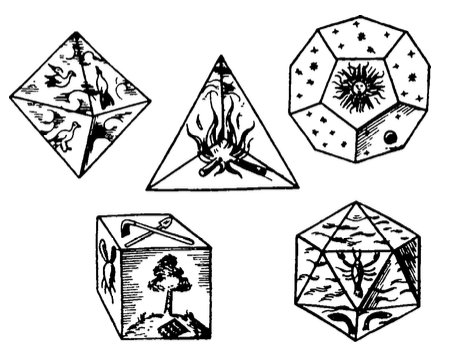
\includegraphics[width=10cm]{images/polyeder/platonic_solids.png}
\caption{Zeichnung der Platonischen Körper von Johannes Kepler aus \cite{cromwell_polyhedra_1997}. Obere Reihe (v.l.n.r.): \textit{Oktaeder}, \textit{Tetraeder}, \textit{Dodekaeder}. Untere Reihe (v.l.n.r.): \textit{Hexaeder}, \textit{Ikosaeder}.}
\label{fig:platonicsolids}
\end{figure}

\subsubsection{Polyeder}
Bevor wir die Besonderheiten der Symmetrie untersuchen, müssen wir klären, was genau ein Polyeder im mathematischen Sinne definiert. Ein Polyeder (von griechisch \textit{poly} für „viel“ und \textit{hedra} für „Sitz“ oder „Fläche“) ist ein dreidimensionaler Körper, dessen Oberfläche aus ebenen Polygonen (Vielecken) besteht. Nach Cromwell lässt sich ein Polyeder als eine Ansammlung von Flächen beschreiben, die so miteinander verbunden sind, dass sie einen abgeschlossenen Raumteil umschliessen. Dabei müssen zwei wesentliche Bedingungen erfüllt sein:

\begin{itemize}
    \item Jede Kante gehört zu genau zwei Flächen.
    \item Der Körper ist zusammenhängend: Man kann von jeder Fläche zu jeder anderen gelangen, indem man über die Kanten wandert.
\end{itemize}

Die Schnittpunkte, an denen mindestens drei Flächen (und damit mindestens drei Kanten) aufeinandertreffen, bezeichnen wir als Ecken. Ein Tetraeder besitzt beispielsweise 6 Kanten und 4 Ecken (siehe Abbildung \ref{fig:tetraeder}).

\begin{figure}[htp]
\centering
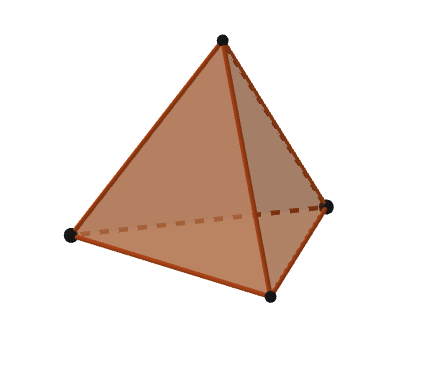
\includegraphics[width=0.4\textwidth]{images/polyeder/tetraeder.png}
\caption{Reguläres Tetraeder.}
\label{fig:tetraeder}
\end{figure}



Alltagsbeispiele für Polyeder sind etwa Pakete oder würfelförmige Regale. Sobald jedoch gekrümmte Begrenzungsflächen vorhanden sind – wie bei einer Kugel oder einer Getränkedose –, handelt es sich nicht mehr um ein Polyeder (siehe Abbildung \ref{fig:auswahl_polyeder}).

\begin{figure}[htbp]
     \centering
     \begin{subfigure}[b]{0.3\textwidth}
         \centering
         \includegraphics[width=\textwidth]{images/polyeder/kuppelhaus_düsseldorf.jpg}
         \caption{Kuppelhaus des botanischen Gartens in Düsseldorf.}
         \label{fig:kuppelhaus_düsseldorf}
     \end{subfigure}
     \hfill
     \begin{subfigure}[b]{0.3\textwidth}
         \centering
         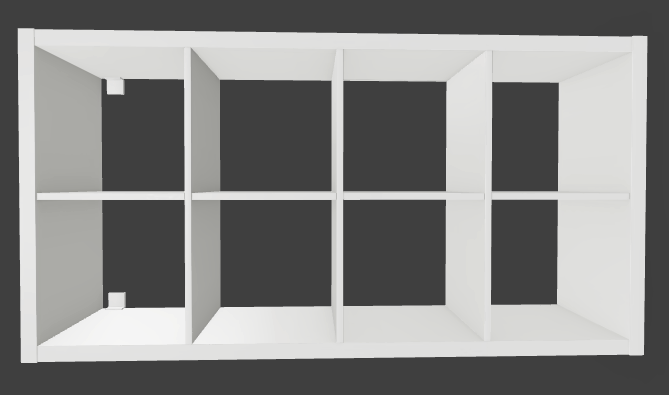
\includegraphics[width=\textwidth]{images/polyeder/kallax_ikea.png}
         \caption{Regalsystem.}
         \label{fig:kallaxikea}
     \end{subfigure}
     \hfill
     \begin{subfigure}[b]{0.3\textwidth}
         \centering
         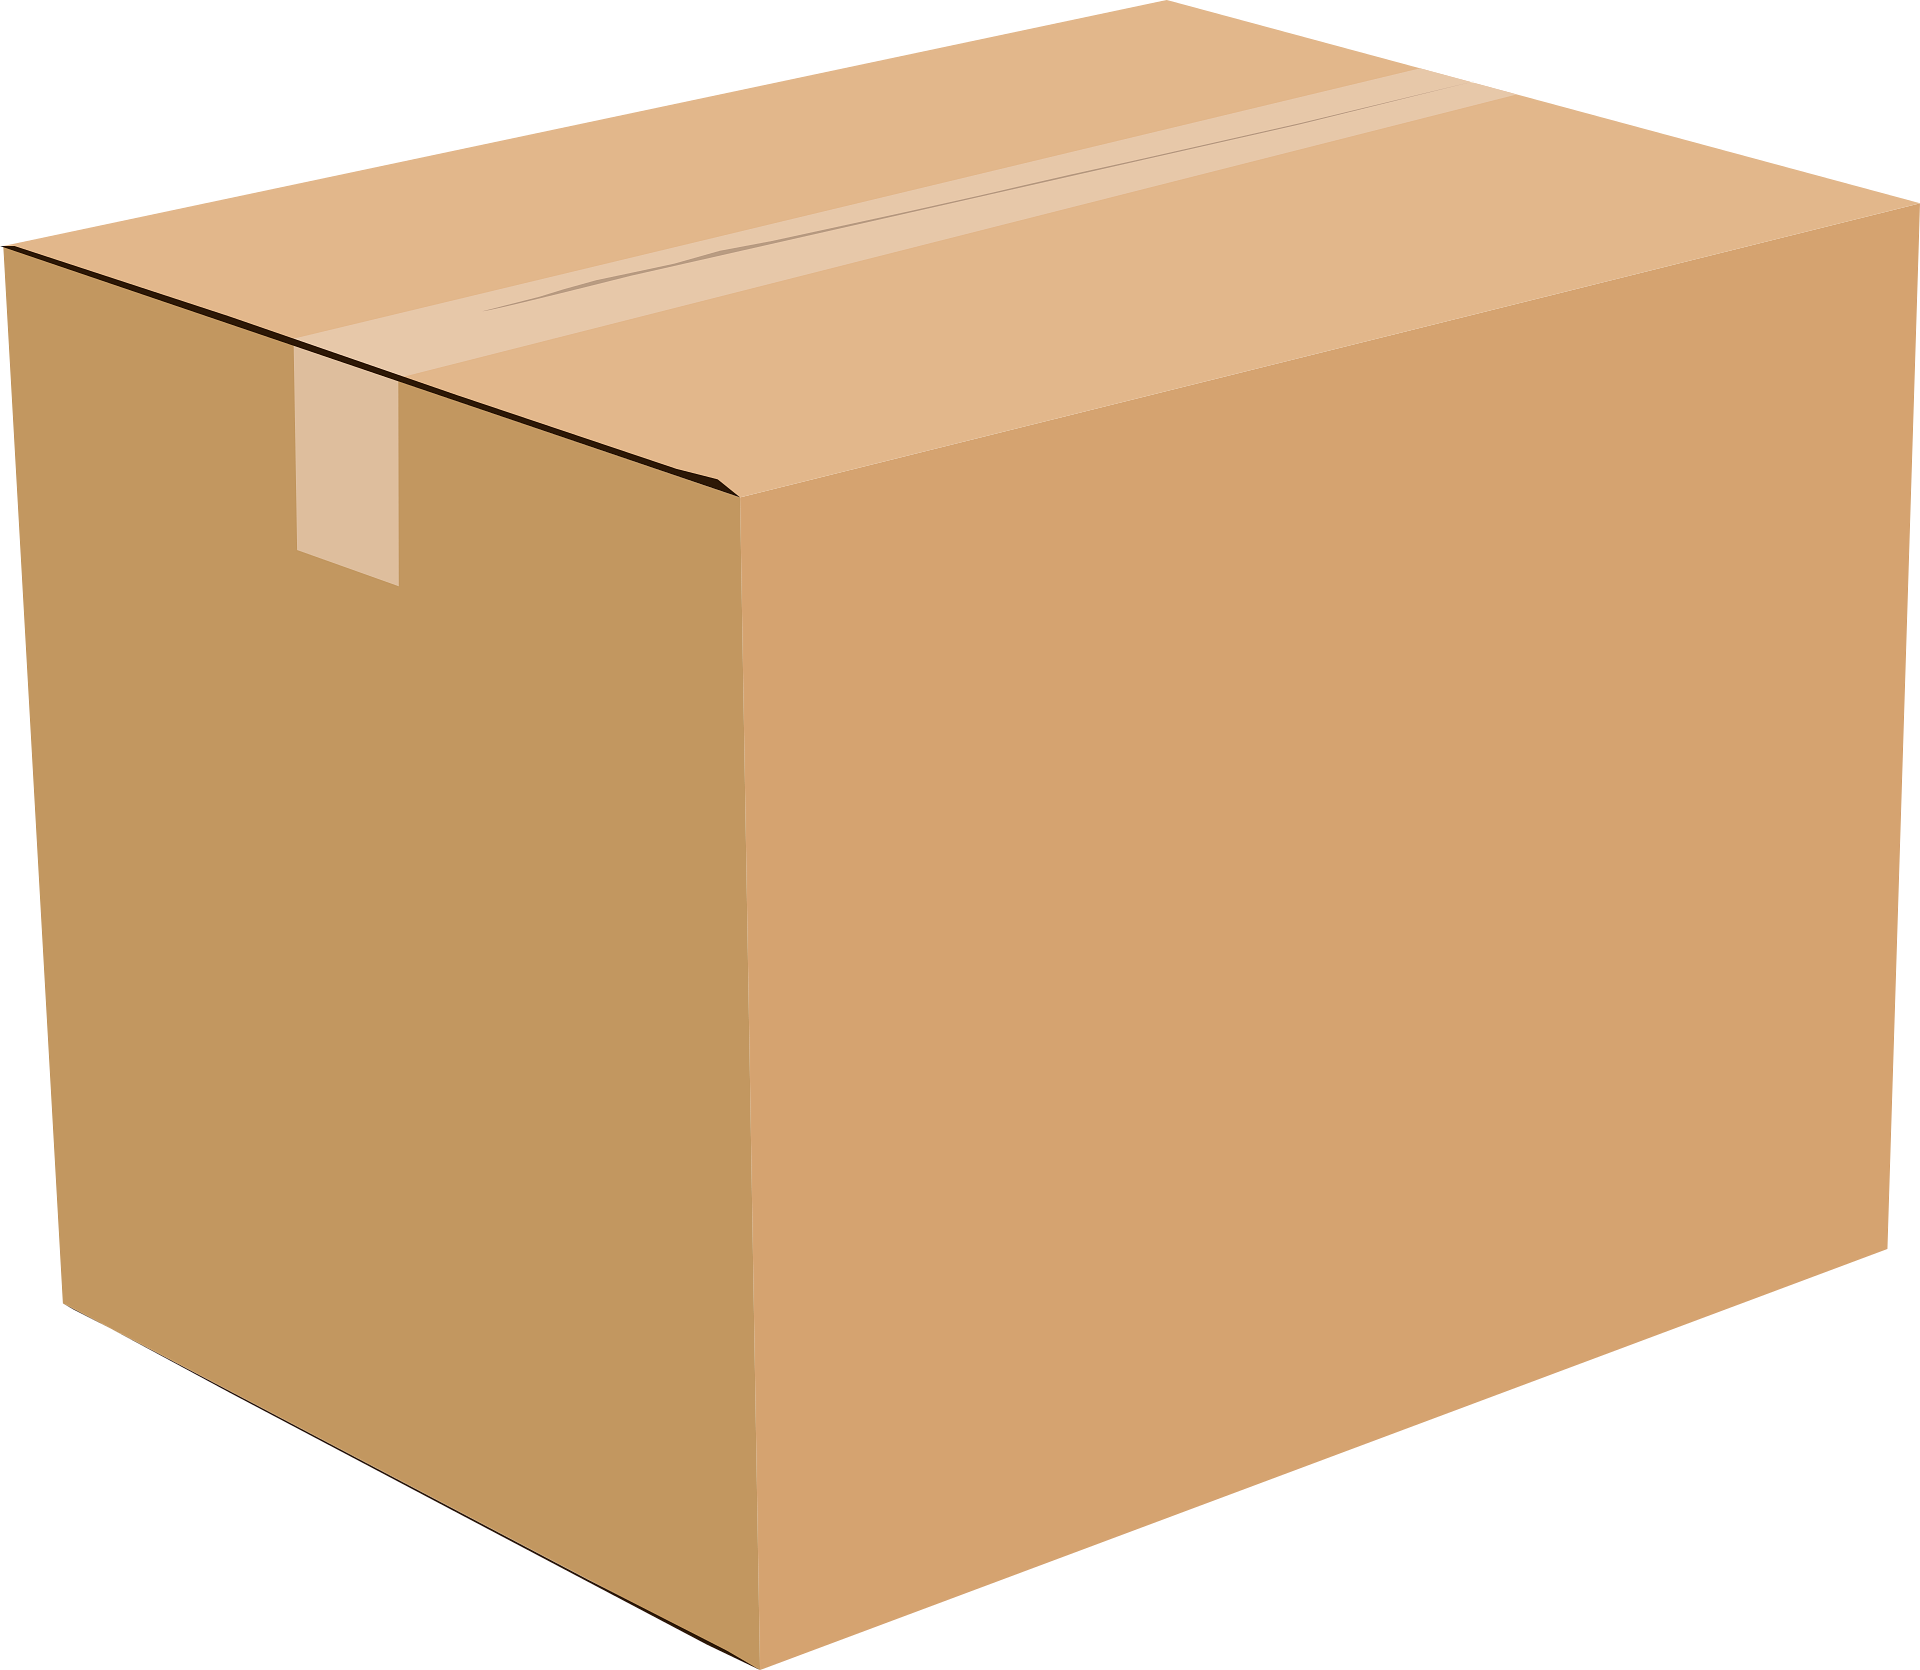
\includegraphics[width=\textwidth]{images/polyeder/paket.png}
         \caption{Quaderförmiges Paket.}
         \label{fig:Paket}
     \end{subfigure}
        \caption{Beispiele für Polyeder im Alltag und in der Architektur.}
        \label{fig:auswahl_polyeder}
\end{figure}

Damit ein Polyeder als \textit{regulär} eingestuft wird, müssen laut Coxeter zwei strenge Anforderungen an seine Regelmässigkeit erfüllt sein:

\begin{itemize}
    \item \textbf{Flächenregularität}: Alle Seitenflächen sind kongruente, reguläre Vielecke. Dies bedeutet, dass alle Kanten gleich lang und alle Innenwinkel der Flächen identisch sind.
    \item \textbf{Eckenregularität}: An jeder Ecke des Polyeders treffen stets gleich viele Flächen in der immer gleichen Anordnung zusammen.
\end{itemize}

Diese Struktur wird mathematisch durch das Schläfli-Symbol $\{p, q\}$ zusammengefasst. Dabei steht $p$ für die Anzahl der Ecken einer einzelnen Fläche und $q$ für die Anzahl der Flächen, die an einer Ecke zusammentreffen. Ein Würfel besteht aus Quadraten ($p=4$), von denen drei an jeder Ecke zusammenkommen ($q=3$), was zum Symbol $\{4, 3\}$ führt. 

Von diesen regulären Polyedern, auch als Platonische Körper bekannt, existieren exakt fünf:
\begin{itemize}
    \item \textbf{Reguläres Tetraeder}: (griech. \textit{tetra} = vier) Begrenzt von vier regulären Dreiecken.
    \item \textbf{Reguläres Hexaeder}: (griech. \textit{hex} = sechs) Der Würfel, begrenzt von sechs Quadraten.
    \item \textbf{Reguläres Oktaeder}: (griech. \textit{oktō} = acht) Begrenzt von acht regulären Dreiecken.
    \item \textbf{Reguläres Dodekaeder}: (griech. \textit{dōdeka} = zwölf) Begrenzt von zwölf regulären Fünfecken.
    \item \textbf{Reguläres Ikosaeder}: (griech. \textit{eíkosi} = zwanzig) Begrenzt von zwanzig regulären Dreiecken.
\end{itemize}



Es existieren verschiedene Beweise dafür, dass es genau fünf reguläre Polyeder gibt. Ein geometrischer Beweis von Euklid basiert auf den Innenwinkeln der Flächen. Ein weiterer, algebraischer Beweis stammt von Leonhard Euler; dieser nutzt den Polyedersatz und benötigt keine Betrachtung der Winkel. Da diese Beweise für den weiteren Verlauf dieser Arbeit nicht unmittelbar relevant sind, verweisen wir auf die entsprechende Literatur \cite[Kap.~2]{coxeter_regular_polytopes_1973, cromwell_polyhedra_1997}. Im nächsten Abschnitt werden wir uns intensiv mit den Symmetriegruppen dieser Körper beschäftigen.


\subsubsection{Aufgaben}

\begin{exercise} \label{ex:polyederalltag}
    Nennen Sie drei weitere Beispiele für Polyeder aus Ihrem Alltag, die noch nicht im Text erwähnt wurden. Begründen Sie kurz anhand der Definition, warum es sich um Polyeder handelt.
\end{exercise}

\begin{exercise} \label{ex:polyederbeispiele}
    Prüfen Sie anhand der Definition eines Polyeders, ob es sich bei den folgenden Objekten um ein solches handelt:
    \begin{itemize}
        \item[a)] der \textit{Adidas Fevernova} (offizieller Fussball der WM 2002),
        \item[b)] ein klassischer Spielwürfel mit abgerundeten Ecken.
    \end{itemize}
    Begründen Sie Ihre Antwort. Handelt es sich zudem um \textbf{reguläre} Polyeder?
\end{exercise}